\documentclass[11pt, a4paper]{article}
\usepackage[utf8]{inputenc}
\usepackage{amsmath, amssymb}
\usepackage{graphicx}
\usepackage{hyperref}
\usepackage{xcolor}
\usepackage{listings}
\lstset{
    language=Python,
    basicstyle=\ttfamily\small,
    keywordstyle=\color{blue}\bfseries,
    commentstyle=\color{gray}\itshape,
    stringstyle=\color{orange},
    numberstyle=\tiny\color{gray},
    numbers=left,
    stepnumber=1,
    numbersep=8pt,
    frame=single,
    breaklines=true,
    breakatwhitespace=false,
    showstringspaces=false,
    tabsize=4,
    captionpos=b
}
\usepackage{geometry}
\geometry{margin=1in}

\title{EE 325 Digital Signal Processing \\ Assignment 5: System Characterization via z-Transform}
\author{PERERA J.D.T. \\ E/21/291}
\date{\today}

\begin{document}
\maketitle

\section{1. Transfer Function from Difference Equation}
\textbf{System:}
$$y[n] - 1.1y[n-1] + 0.3y[n-2] = x[n] + 0.5x[n-1]$$

\textbf{(a) Derive H(z):}
Taking the z-transform of both sides:
$$Y(z) - 1.1z^{-1}Y(z) + 0.3z^{-2}Y(z) = X(z) + 0.5z^{-1}X(z)$$
$$Y(z) [1 - 1.1z^{-1} + 0.3z^{-2}] = X(z) [1 + 0.5z^{-1}]$$

The transfer function $H(z) = \frac{Y(z)}{X(z)}$ is:
$$H(z) = \frac{1 + 0.5z^{-1}}{1 - 1.1z^{-1} + 0.3z^{-2}}$$

\textbf{(b) Coefficients:}
Expressing in the form $H(z) = \frac{b_0 + b_1 z^{-1} + \dots}{1 + a_1 z^{-1} + a_2 z^{-2}}$:
$$H(z) = \frac{1 + 0.5z^{-1}}{1 - 1.1z^{-1} + 0.3z^{-2}}$$

Coefficients:
\begin{itemize}
    \item Numerator $\{b_k\}$: $b_0 = 1, b_1 = 0.5$
    \item Denominator $\{a_k\}$: $a_0=1, a_1 = -1.1, a_2 = 0.3$
\end{itemize}

\section{2. Pole-Zero Analysis and Stability}

\textbf{(a) Poles and Zeros:}
Zeros (roots of numerator $1 + 0.5z^{-1}$):
$$1 + 0.5z^{-1} = 0 \implies z = -0.5$$
Zero at $z = -0.5$.

Poles (roots of denominator $1 - 1.1z^{-1} + 0.3z^{-2}$):
Multiply by $z^2$: $z^2 - 1.1z + 0.3 = 0$.
Roots using quadratic formula:
$$z = \frac{1.1 \pm \sqrt{1.1^2 - 4(1)(0.3)}}{2} = \frac{1.1 \pm \sqrt{1.21 - 1.2}}{2} = \frac{1.1 \pm \sqrt{0.01}}{2}$$
$$z = \frac{1.1 \pm 0.1}{2}$$
$p_1 = \frac{1.2}{2} = 0.6$\\
$p_2 = \frac{1.0}{2} = 0.5$

Poles at $z = 0.6$ and $z = 0.5$.

\textbf{(b) Stability:}
A causal LTI system is BIBO stable if all poles lie \textbf{strictly inside the unit circle} ($|p| < 1$).
Here, poles are $0.5$ and $0.6$.
Since $|0.5| < 1$ and $|0.6| < 1$, the system is \textbf{Stable}.

\textbf{(c) System Type:}
The system has poles (denominator order $> 0$), meaning $y[n]$ depends on past outputs. Thus, it has an impulse response of infinite duration. The system is \textbf{IIR (Infinite Impulse Response)}.

\section{3. Frequency Response}
\textbf{Gain Analysis:}
\begin{itemize}
    \item \textbf{DC Gain ($\omega = 0, z = 1$):} \\
    $$H(e^{j0}) = H(1) = \frac{1 + 0.5}{1 - 1.1 + 0.3} = \frac{1.5}{0.2} = 7.5$$ \\
    Magnitude: $20 \log_{10}(7.5) \approx 17.5$ dB.
    
    \item \textbf{Nyquist Gain ($\omega = \pi, z = -1$):} \\
    $$H(e^{j\pi}) = H(-1) = \frac{1 - 0.5}{1 + 1.1 + 0.3} = \frac{0.5}{2.4} \approx 0.208$$ \\
    Magnitude: $20 \log_{10}(0.208) \approx -13.6$ dB.
\end{itemize}

\textbf{Pole-Zero Influence:}
\begin{itemize}
    \item The poles are at $z=0.5, 0.6$. These are positive real poles, closest to the unit circle at $\omega=0$ ($z=1$).
    \item This proximity to $\omega=0$ causes a \textbf{rise in magnitude at low frequencies} (Low Pass behavior), which explains the high DC gain.
    \item The zero at $z=-0.5$ is on the negative real axis ($\omega=\pi$). This suppresses high frequencies, contributing to the low magnitude at $\pi$.
\end{itemize}

\begin{figure}[h]
    \centering
    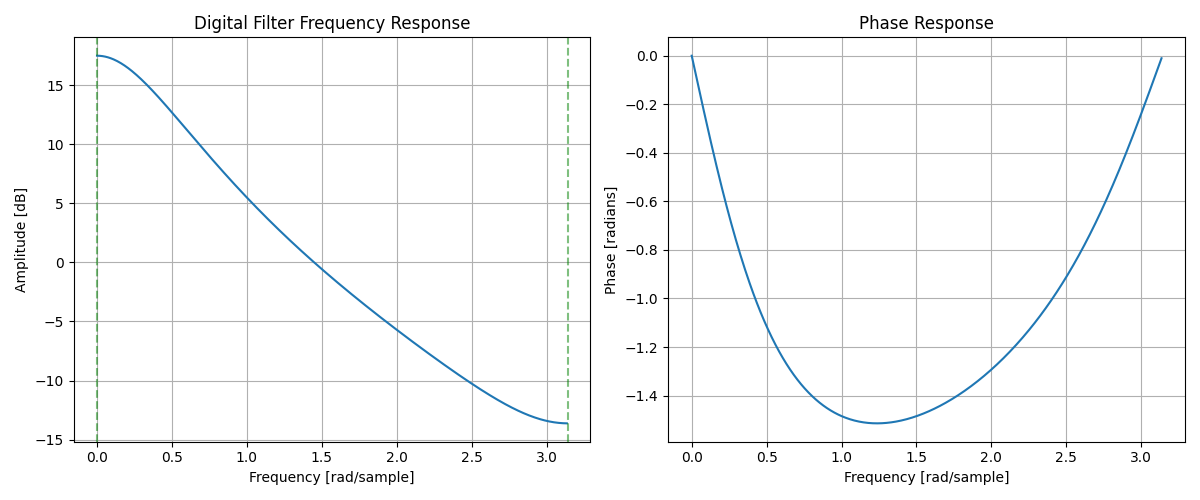
\includegraphics[width=0.8\textwidth]{frequency_response.png}
    \caption{Frequency Response}
    \label{fig:freq_res}
\end{figure}

\begin{figure}[h]
    \centering
    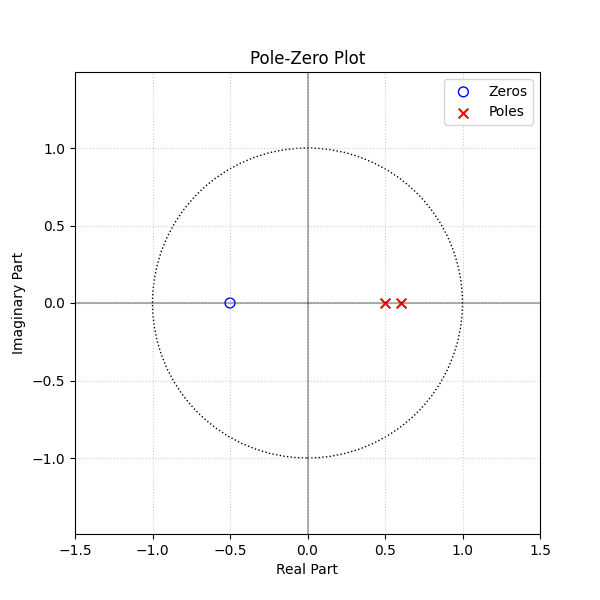
\includegraphics[width=0.8\textwidth]{pole_zero_plot.png}
    \caption{Pole-Zero Plot}
    \label{fig:pz_plot}
\end{figure}

\appendix
\section{Python Source Code}
\textbf{File:} \texttt{freq\_response\_plot.py}
\begin{lstlisting}[caption={System Analysis via z-Transform and Frequency Response -- Assignment 5}]
import numpy as np
import matplotlib.pyplot as plt
from scipy import signal

def analyze_system():
    b = [1, 0.5]
    a = [1, -1.1, 0.3]
    
    # Q2: Pole-Zero Analysis
    z, p, k = signal.tf2zpk(b, a)
    print("--- Pole-Zero Analysis ---")
    print(f"Zeros: {z}")
    print(f"Poles: {p}")
    is_stable = np.all(np.abs(p) < 1)
    print(f"System Stable? {is_stable} (Max pole magnitude: {np.max(np.abs(p)):.4f})")
    
    # Q3: Frequency Response
    w, h = signal.freqz(b, a)
    mag = 20 * np.log10(np.abs(h))
    phase = np.angle(h)
    dc_gain = np.abs(h[0])
    nyquist_gain = np.abs(h[-1])
    print("\n--- Frequency Response Analysis ---")
    print(f"DC Gain (w=0): {dc_gain:.4f} ({20*np.log10(dc_gain):.4f} dB)")
    print(f"Nyquist Gain (w=pi): {nyquist_gain:.4f} ({20*np.log10(nyquist_gain):.4f} dB)")
    
    plt.figure(figsize=(12, 5))
    plt.subplot(1, 2, 1)
    plt.plot(w, mag)
    plt.title('Digital Filter Frequency Response')
    plt.ylabel('Amplitude [dB]')
    plt.xlabel('Frequency [rad/sample]')
    plt.grid(True)
    
    plt.subplot(1, 2, 2)
    plt.plot(w, phase)
    plt.title('Phase Response')
    plt.ylabel('Phase [radians]')
    plt.xlabel('Frequency [rad/sample]')
    plt.grid(True)
    plt.tight_layout()
    plt.savefig('frequency_response.png')
    print("Plot saved to frequency_response.png")
    
    plt.figure(figsize=(6, 6))
    plt.scatter(np.real(z), np.imag(z), s=50, marker='o', edgecolors='b', facecolors='none', label='Zeros')
    plt.scatter(np.real(p), np.imag(p), s=50, marker='x', color='r', label='Poles')
    circle = plt.Circle((0,0),1, fill=False, linestyle='dotted', color='k')
    plt.gca().add_patch(circle)
    plt.axhline(0, color='k', alpha=0.3)
    plt.axvline(0, color='k', alpha=0.3)
    plt.grid(True, linestyle=':', alpha=0.6)
    plt.title('Pole-Zero Plot')
    plt.xlabel('Real Part')
    plt.ylabel('Imaginary Part')
    plt.legend()
    plt.axis('equal')
    plt.xlim([-1.5, 1.5])
    plt.ylim([-1.5, 1.5])
    plt.savefig('pole_zero_plot.png')
    print("Plot saved to pole_zero_plot.png")

if __name__ == "__main__":
    analyze_system()
\end{lstlisting}

\end{document}
